% Auto-generated TikZ figure for warm-start loss frontier with per-scale fits
\documentclass[tikz]{standalone}
\usepackage{pgfplots}
\pgfplotsset{compat=1.18}
\begin{document}
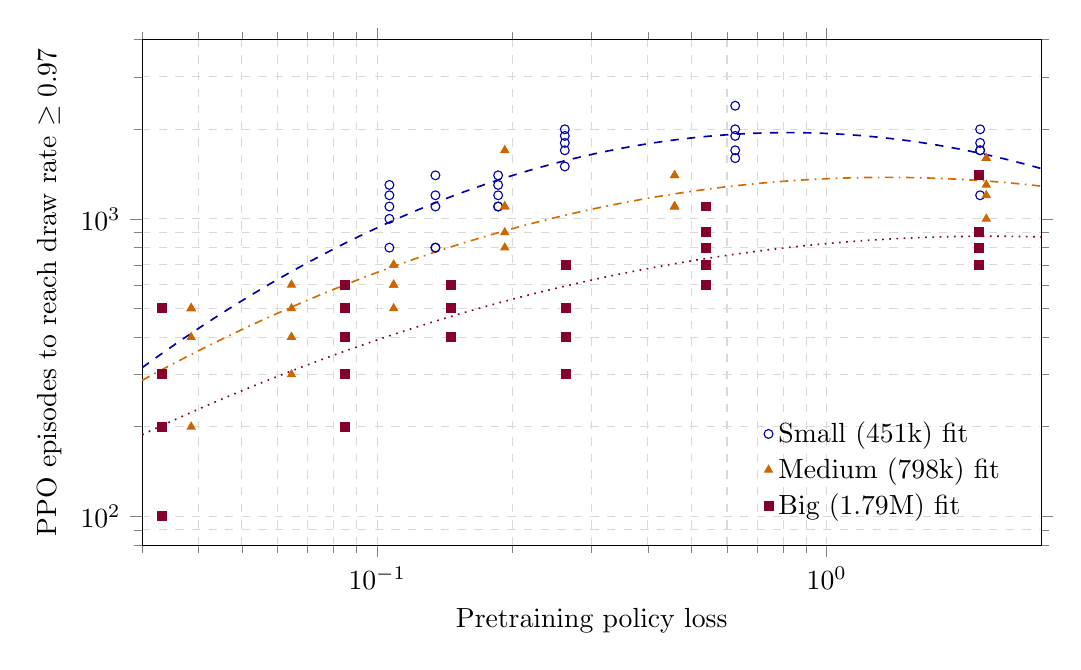
\begin{tikzpicture}
  \begin{axis}[
    width=13cm,
    height=8cm,
    xlabel={Pretraining policy loss},
    ylabel={PPO episodes to reach draw rate $\ge 0.97$},
    xmode=log,
    ymode=log,
    xmin=0.03, xmax=3,
    ymin=80, ymax=4000,
    grid=both,
    grid style={dashed, gray!30},
    legend style={at={(0.97,0.03)}, anchor=south east, draw=none, fill=none, font=\normalsize},
    legend cell align=left,
    axis background/.style={fill=white},
    tick align=outside,
  ]
  % scatter points per capacity
  % Auto-generated scatter data for warm-start loss frontier figure

% Small (451k) scatter data
\addplot[only marks, mark size=1.6pt, color=blue!65!black, mark=o] table[row sep=\\]{%
0.106436 800\\
0.106436 1000\\
0.106436 1100\\
0.106436 1200\\
0.106436 1300\\
0.134742 800\\
0.134742 800\\
0.134742 1100\\
0.134742 1200\\
0.134742 1400\\
0.185773 1100\\
0.185773 1100\\
0.185773 1200\\
0.185773 1300\\
0.185773 1400\\
0.261355 1500\\
0.261355 1700\\
0.261355 1800\\
0.261355 1900\\
0.261355 2000\\
0.625703 1600\\
0.625703 1700\\
0.625703 1900\\
0.625703 2000\\
0.625703 2400\\
2.193770 1200\\
2.193770 1700\\
2.193770 1700\\
2.193770 1800\\
2.193770 2000\\
};

% Medium (798k) scatter data
\addplot[only marks, mark size=1.6pt, color=orange!80!black, mark=triangle*] table[row sep=\\]{%
0.038564 200\\
0.038564 400\\
0.038564 500\\
0.038564 500\\
0.038564 500\\
0.064462 300\\
0.064462 400\\
0.064462 400\\
0.064462 500\\
0.064462 600\\
0.108793 500\\
0.108793 600\\
0.108793 600\\
0.108793 700\\
0.108793 700\\
0.192195 800\\
0.192195 900\\
0.192195 1100\\
0.192195 1100\\
0.192195 1700\\
0.458714 1100\\
0.458714 1100\\
0.458714 1100\\
0.458714 1400\\
0.458714 1400\\
2.263852 1000\\
2.263852 1200\\
2.263852 1300\\
2.263852 1600\\
2.263852 1600\\
};

% Big (1.79M) scatter data
\addplot[only marks, mark size=1.6pt, color=purple!70!black, mark=square*] table[row sep=\\]{%
0.033204 100\\
0.033204 100\\
0.033204 200\\
0.033204 300\\
0.033204 500\\
0.084617 200\\
0.084617 300\\
0.084617 400\\
0.084617 500\\
0.084617 600\\
0.146177 400\\
0.146177 500\\
0.146177 500\\
0.146177 600\\
0.146177 600\\
0.263279 300\\
0.263279 400\\
0.263279 500\\
0.263279 700\\
0.263279 700\\
0.537664 600\\
0.537664 700\\
0.537664 800\\
0.537664 900\\
0.537664 1100\\
2.181965 700\\
2.181965 700\\
2.181965 800\\
2.181965 900\\
2.181965 1400\\
};

  % per-capacity fits
  \addplot[domain=0.03:3, samples=200, semithick, color=blue!70!black, dashed] {exp(-0.166022829*(ln(x))^2 -0.065211060*ln(x) + 7.568635609)};
  \addlegendentry{Small (451k) fit}
  \addplot[domain=0.03:3, samples=200, semithick, color=orange!85!black, dashdotted] {exp(-0.107978258*(ln(x))^2 +0.066385081*ln(x) + 7.218350135)};
  \addlegendentry{Medium (798k) fit}
  \addplot[domain=0.03:3, samples=200, semithick, color=purple!70!black, dotted] {exp(-0.081396337*(ln(x))^2 +0.136342388*ln(x) + 6.716066562)};
  \addlegendentry{Big (1.79M) fit}
  \end{axis}
\end{tikzpicture}
\end{document}
